\documentclass{article}

% \usepackage[utf8]{inputenc} 
\usepackage{a4wide}
\usepackage[left=20mm,top=10mm,bottom=0mm,right=20mm,headheight=15mm,headsep=10mm,footskip=10mm]{geometry}
\usepackage{selinput}
% \usepackage[latin1]{inputenc}
\usepackage[ngerman,naustrian]{babel}
\usepackage{lmodern}
\usepackage[T1]{fontenc}
\usepackage{helvet}
\renewcommand{\familydefault}{\sfdefault}
\usepackage{ulem}
\usepackage{hyperref}
\usepackage{here}
\usepackage[pdftex]{graphicx}
% \usepackage{amsthm}
% \usepackage{gensymb}
% \usepackage{fancyhdr}
% \pagestyle{fancy} 
% \usepackage{xcolor}
\usepackage{longtable}
\usepackage{hhline}
\usepackage[table]{xcolor}
% \usepackage{tabularx}
\usepackage{multicol}
\usepackage{graphicx}

\renewcommand{\familydefault}{\sfdefault}

\begin{document}

\pagestyle{empty}

	\begin{tabular}{|l|l|ll|}
	\hline
	Studis:	Simon Steidl	& 1te Ü aus RTO1UE				& 07.10 und 14.10.2020		& \\
	\hspace{0.2\textwidth}	& \hspace{0.5\textwidth}	& \hspace{0.2\textwidth}	& \\
	Florian Hinterleitner	& Timing of several Tasks 	& FH Hagenberg	& \\
	\hline
	\end  {tabular}

		% \sffamily


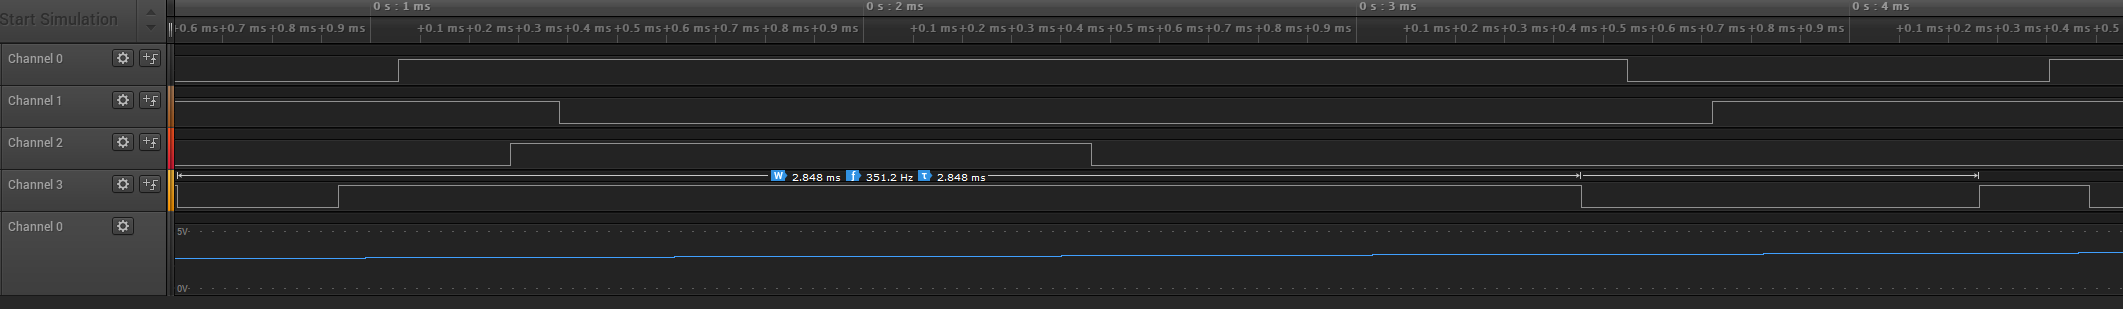
\includegraphics[width=.8\textwidth]{Saleae_nonense}
% screenshots
% Timing-tabelle
% 

\end{document}